Prior work has shown that graph-based approaches can be effective for vulnerability detection:
    they leverage code structure (CPGs, PDGs) to identify anomalous patterns indicative of vulnerabilities,
        but they typically require large amounts of labeled data and struggle to generalize to novel vulnerability types.

Our proposal: a retrieval-augmented approach that leverages a knowledge base of known vulnerability patterns
    to improve precision when ranking candidate sinks, even with limited training data.

Phase 1 — Feasibility (AutoPatch dataset):
    used AutoPatch as a controlled dataset to validate the concept and define baselines
    baselines: structure-only embeddings (NetLSD + WL + GIN) vs. CodeBERT
    result: comparable retrieval performance between CodeBERT and combined structural embeddings
        → structural graph representations capture vulnerability patterns as effectively as pretrained code models

Phase 2 — Generalization (CVEfixes dataset):
    question: does the approach generalize to real-world, more complex vulnerabilities?
    initial results on CVEfixes are weaker — likely due to greater code diversity and patch complexity
    deeper analysis needed to isolate failure modes (embedding collapse, CWE coverage gaps, etc.)

Phase 3 — Candidate sink ranking (current direction):
    leverage Joern static analysis to identify candidate sinks in CVEfixes code
    apply our KB-guided retrieval to rank candidates and reduce false positives
    goal: demonstrate that knowledge-base retrieval adds precision on top of static analysis

% =============================================================================
% RUNNING EXAMPLE: CVE-2024-56605 — Use-After-Free in Linux Bluetooth L2CAP
% =============================================================================

Running Example — CVE-2024-56605 (CWE-416: Use After Free):

    Simplified vulnerable code:
    \begin{verbatim}
    struct sock *alloc_socket(struct socket *sock) {
        struct sock *sk;
        struct chan *ch;

        sk = sk_alloc();          // (1) allocate socket
        if (!sk) return NULL;

        sock->sk = sk;            // (2) store pointer in parent

        ch = chan_create();        // (3) allocate channel
        if (!ch) {
            sk_free(sk);          // (4) free socket on failure
            return NULL;          // BUG: sock->sk still points to freed memory
        }
        return sk;
    }
    \end{verbatim}

    The fix (one line):
    \begin{verbatim}
        if (!ch) {
            sk_free(sk);
            sock->sk = NULL;      // FIX: nullify dangling pointer
            return NULL;
        }
    \end{verbatim}

    Intuition: after sk_free(sk), the alias sock->sk becomes a dangling pointer.
    Any subsequent access via sock->sk is a use-after-free.

% --- CPG Visualization (Code Property Graph) ---
% Generated by Joern (joern-parse + joern-export --repr cpg14)
% Source files:
%   - cpg_example.dot   → annotated CPG (CFG + DDG edges, vulnerability highlighted)
%   - cpg_example.pdf   → rendered PDF (for inclusion in Beamer)
%   - joern_cfg_raw.pdf → raw Joern CFG output (unmodified)
%   - export_cpg14/1-cpg.dot → full CPG14 DOT from Joern (AST + CFG + DDG + CDG)

    CPG for this snippet (generated by Joern, annotated):
    % 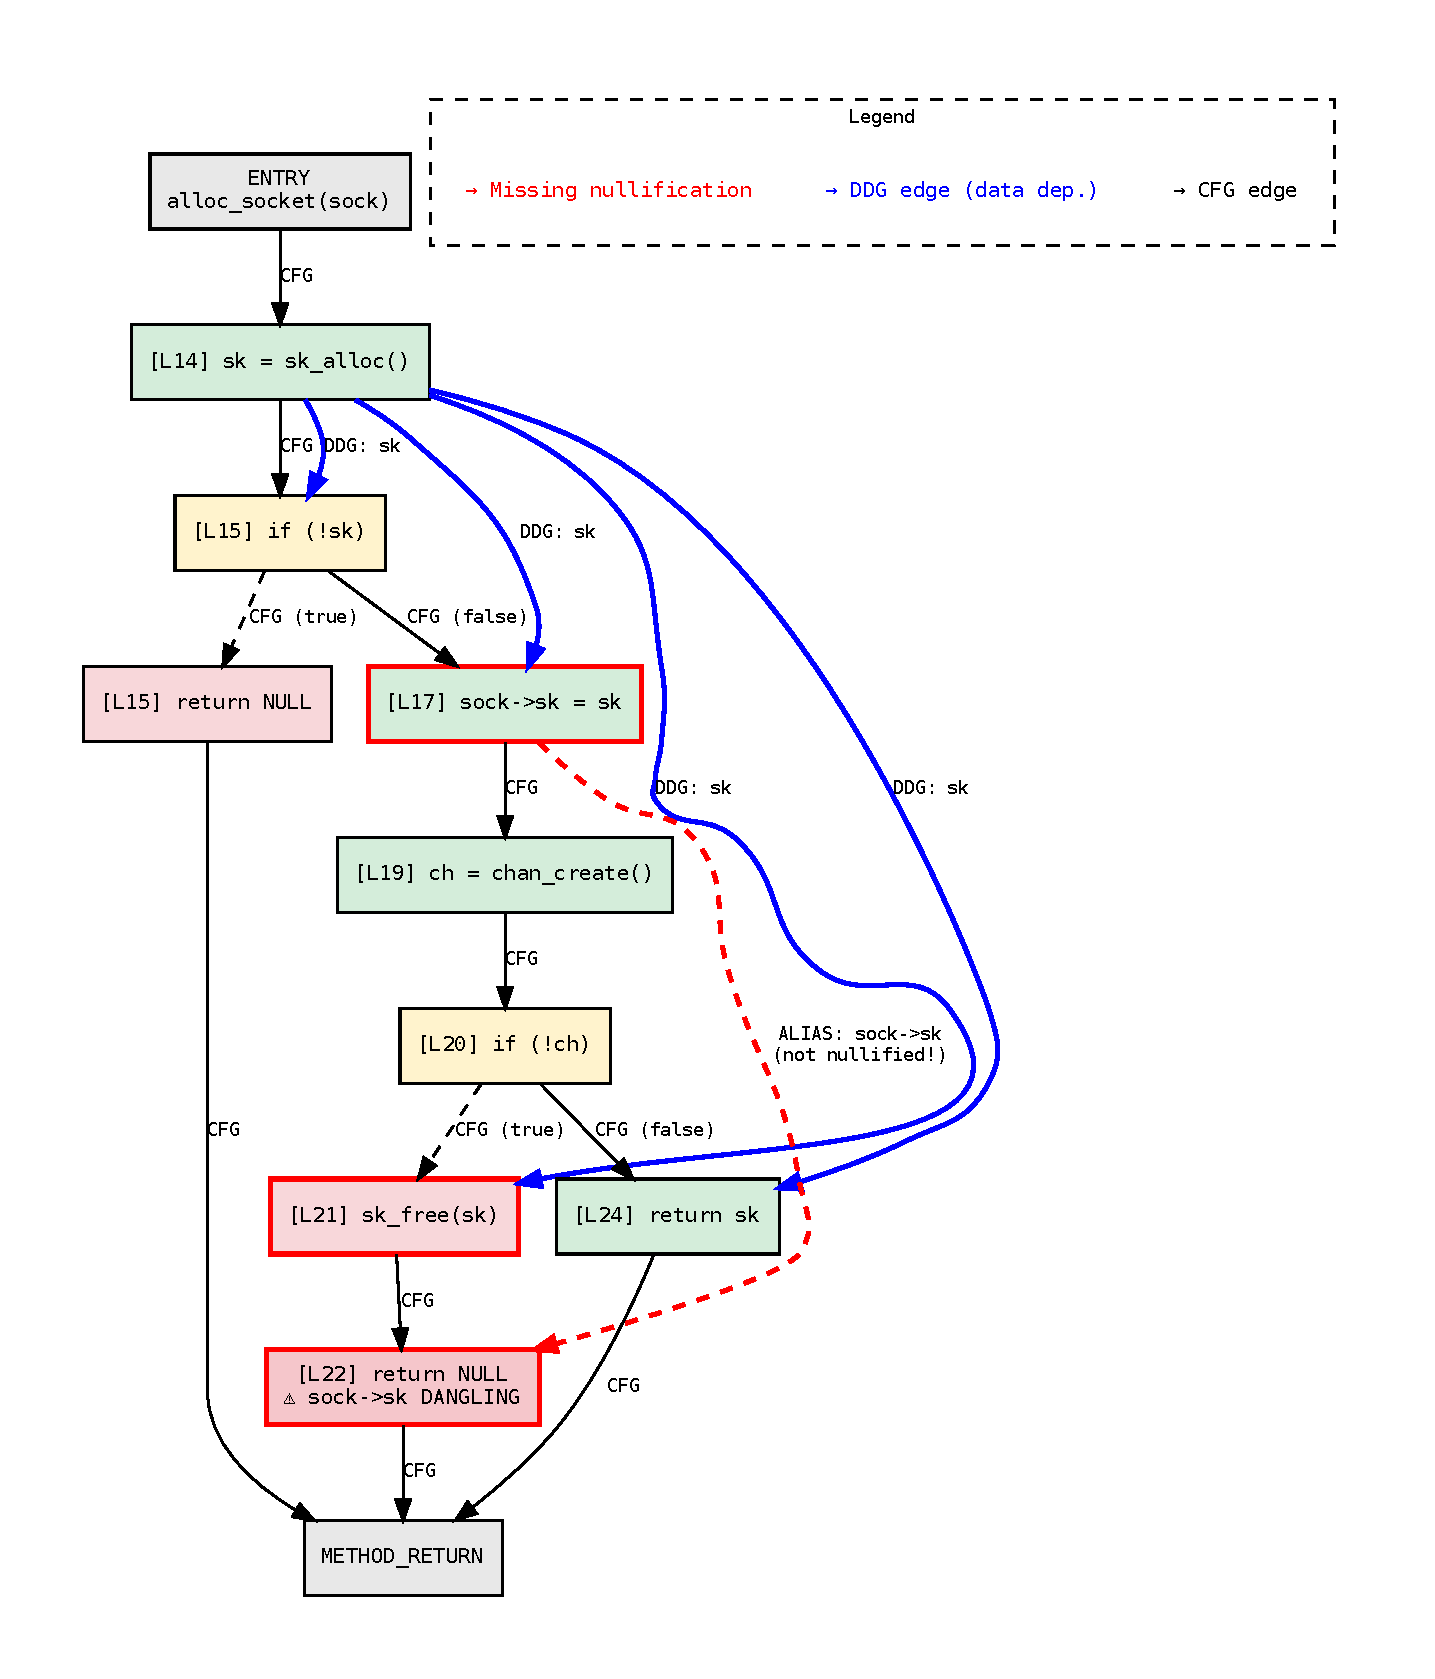
\includegraphics[width=\textwidth]{cpg_example.pdf}

    Key observations from the real CPG:
        - CFG shows two branches at "if (!ch)": one to sk_free → return NULL, one to return sk
        - DDG shows sk flows from sk_alloc() → {check_sk, assign_alias, sk_free, return sk}
          i.e., the same variable reaches both the alias creation (sock->sk = sk) and the free
        - CDG shows sk_free is control-dependent on the (!ch) condition
        - MISSING: no DDG edge from sk_free back to sock->sk (no nullification)
          → this is the structural signature of the UAF

% --- Joern Query ---
% Full query saved in: joern_uaf_query.sc

    Joern query to find this pattern (free without nullification of alias):

    \begin{verbatim}
    // Find free() calls where the freed pointer has a dangling alias
    val uafCandidates = cpg.call.name(".*free.*")
      .where(_.argument(1).isIdentifier)
      .map { freeCall =>
        val freedVar = freeCall.argument(1).code
        val method   = freeCall.method

        // Find aliases: assignments where freedVar is the source
        // e.g., sock->sk = sk  →  "sock->sk" is an alias of sk
        val aliases = method.assignment
          .where(_.source.isIdentifier.name(freedVar))
          .target.code.l

        // Check which aliases are nullified AFTER the free
        val freeLineNo = freeCall.lineNumber.get
        val nullified = method.assignment
          .where(_.lineNumber.map(_ > freeLineNo))
          .where(_.source.code("NULL|nullptr|0"))
          .target.code.l

        // Report: aliases NOT nullified → potential UAF
        val dangling = aliases.filterNot(nullified.contains)
        (freeCall, dangling)
      }
      .filter(_._2.nonEmpty)
    \end{verbatim}

    Expected output on our example:
    \begin{verbatim}
    [UAF] sk_free(sk) at line 21 — dangling aliases: sock->sk
    \end{verbatim}

% --- Challenges (motivating KB-guided ranking) ---

    Challenges this example illustrates:

    1. Joern finds candidates but produces false positives:
        - not every free() without NULL is a bug (e.g., if function returns immediately
          and no caller accesses the alias → no actual UAF)
        - context-sensitivity is hard: sock_init_data() internally sets sock->sk = sk,
          so the alias creation is hidden behind a function call

    2. CPG captures structure, but interpretation requires pattern knowledge:
        - the graph encodes the data flow faithfully
        - but detecting that this specific shape is dangerous requires knowing
          the "free-without-nullify-alias" pattern from prior vulnerabilities

    3. This motivates our approach:
        - Joern (static analysis) → high recall, generates candidate sinks
        - KB retrieval (graph similarity) → high precision, ranks candidates
          by similarity to known vulnerability patterns in the knowledge base
        - together: reduce FP while maintaining coverage